\section{Resource-centered Methods}\label{section:resource_centered_methods}

In this section, we present a collection of  \textit{resource-centered} methods for tag prediction. They are so called because they leverage only resource-specific information in order to predict what tags should be assigned to a new, unlabelled resource. In other words, all prediction are of \textit{unpersonalized} nature.

We note that, although our problem domain only includes textual documents, we chose to also mention in this section approaches used in other domains, such as audio, video and images. This is because we are mostly interested in how these approaches work irrespective of the choice of features used.

\subsection{Association Rule Mining}

\textit{Association rule mining}\footnote{Alternatively, \textit{Association rule learning}.} refer to methods whereby one extracts rules and regularities from event databases \citep{agrawal_etal_93}. For example, the rule $\{\textnormal{Beer,Bread}\} \rightarrow \{\textnormal{Milk}\}$, when referring to a database of supermarket items, may indicate that Beer and Bread jointly \textit{co-occur} very frequently with Milk, suggesting a possible relationship between the two.

In one of the earlier papers on social tag prediction, HEYMANN et al. \citeyearpar{heymann_etal_2008} have applied \textit{association rules} of the form $X \rightarrow Y$ (where $X$ and $Y$ are tagsets) in order to expand the set of tags given to a resource. Using techniques such as \textit{Market Basket Analysis}, the authors derive association rules of length 4 and below, using a certain level of support\footnote{A rule's \textit{support} equals the number of examples where both $X$ and $Y$ are present.} as threshold to remove overly noisy rules.

The authors report \citep{heymann_etal_2008} that a surprisingly high number of high quality rules can be found (such as those representing \textit{type-of} relationships and synonyms). Furthermore, the added tags help increase precision and recall for user queries, when the result sets are augmented to include documents tagged with those tags.

The authors also claim that using larger and larger rules would probably increase performance, but computational complexity quickly become prohibitive.\footnote{Note that this method assumes that a resource already has some tags assigned to it. These are then used to predict another set of tags. This is sometimes called \textbf{tag-set expansion} in order to differentiate it from methods that do not make this assumption.}

Another approach involving association rules was put forward by \cite{vanleeuwen_puspitaningrum_2012}. They acknowledge the fact that gains in performance brought about by using larger rules come at a high cost in terms of processing time. They, however, suggest that a compromise can be achieved by choosing a carefully selected set of association rules, such that performance is increased at a lower cost.

Their approach works by using a compression mechanism to efficiently compute expanded tagsets for any given tagset. It computes the most suitable expanded tagsets ranked by support.\footnote{The support for a given tagset is simply the number of times that particular tagset was assigned to a resource in the system.}

\subsection{Content-based tag propagation}

Here we provide a basic overview of methods which, in one way or another, use the content-based similarity to propagate tags from labelled instances to unlabelled ones.

In the first approach, \cite{sordo_etal_2007} have used both first-order (stylistic) and second-order (mood-based, extracted from the stylistic ones) features and a neighbours-based similarity measure to propagate labels from labelled audio pieces to unlabelled ones.

They reported good results for the approach, as measured by rank-based metrics such as Spearman's rank and Precision@$k$. They claim that ignoring tags with too few assignments improves results and that sometimes using more neighbors is beneficial, while sometimes it's harmful.

It should be noted here that this work was not run on a broad folksonomy, since all examples were annotated by a single person.

Another interesting example is that of \cite{moxley_etal_2008}. Their approach uses many feature \textit{modalities} to represent a resource (in this case, videos). In other words, they use multiple sources of information to build a feature vector, namely text information from the video transcripts, image information from video snapshots and concept information from external source.

They report good results using set-based performance metrics (slight variants of precision and recall). Furthermore, they claim that using an average of features built from multiple modalities helps suppress the effect of noisy information.

In \cite{guillaumin_etal_2009}, the authors propose a weighted neighbor approach where one can choose an arbitrary distance measure (i.e. Euclidean, Manhattan, etc) one wishes to use to measure similarity between resource representations. Then, the optimal weights for each resource are found via the optimization of a custom loss function that encodes the accuracy each individual tag prediction. 

In other words, the dataset is used to inform the decision on what weights to use for each resource. This will, in turn, define to what extent tag assignments for each resource will influence those of its neighbors.

This approach has been called \textit{metric learning} and, according to the authors, it has been used in the past in other contexts.

In \cite{li_etal_2009}, the authors have approached the problem from a slightly different angle. Although they have also used content-based similarity to search for neighbors, the weight given to each tag is not just proportional to the similarity between each pair of neighbors; it also incorporates a term that normalizes each tag according to the tag's \textit{prior}, i.e. the overall frequency of a given tag in the whole dataset.

By using rank-based metrics such as Precision@$k$ and Mean Average Precision (MAP), they report that their method consistently outperforms approaches that do not take a tag's overall prior into account.

In conclusion, two common themes in such \textit{content-based} tag propagation approaches seem to be \textbf{a)} designing similarity measures and other ways to retrieve similar resources given a query resource and \textbf{b)} once the neighbor resources are found, find meaningful ways to weigh the contribution given by each neighbor in order to predict tags for the query resource. 

\subsection{Resource-based tag propagation}

In this subsection, we will talk about methods which use information \textit{about} the resource (other than its contents encoded as features) to build representations for these resources. These representations are then used in neighbor-based algorithms for actual classification.

\cite{auyeung_etal_2009} propose a slightly different approach. They encode each resource as a vector over the space of the full tag vocabulary, so that it resembles a bag-of-words approach, using tags instead of terms in the document. Similarity between resources is then calculated via simple measures like cosine similarity.

The authors report above-benchmark performance when using the described approach to predict tags for unlabelled examples. Metrics used to for gauging performance include Precision@$k$ and NDCG.


\subsection{Multi-label Classification/Ranking}\label{subsection:classification_vs_ranking}

Since resources in an STS can be assigned multiple tags, it is natural to model this problem as a \textit{Multi-label Classification} (MLC) problem.

Multi-label learning\footnote{Not to be confused with \textit{multi-class} classification.} (\cite{tsoumakas_katakis_2007}) refers to learning from data that is multi-labelled, that is, data where each example has not just a single label\footnote{Problems where each example has a single label are, unsurprisingly, referred to as \textit{single-label} classification in MLC literature} but multiple ones.

A more particular approach, generally called \textit{Multi-label Ranking}, refers (\cite{illig_etal_2011}) to problems where not only do instances have multiple labels associated with them, but every label also has a \textit{rank}; in other words, each label assignment also carries a weight, so that labels assigned to a particular example may be ranked with respect to the weight each label has. This is in contrast with regular multi-label classification, where labels are represented with a binary vector, making no distinction between labels.\footnote{Although our own method is of the multi-label ranking type, we find it worthwhile to list regular MLC method due to how similar both are.}

\begin{figure}[H]
    \centering
    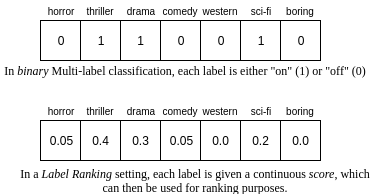
\includegraphics[width=7cm]{chapters/03_related_work/images/label-classification-vs-label-ranking.png}}
    \caption{When each label prediction is given a score, we can choose a threshold $k$ and return only the top $k$ labels, as ranked by score.}
    \label{fig:classification_vs_ranking}
\end{figure}

In \cite{katakis_etal_2008}, the authors have applied multi-label classification to the task of classifying HTML pages and journal abstracts into tags.

The chosen method was to train a binary classifier for each individual label, a meta-classification procedure called \textit{Binary Relevance} \footnote{\textit{Binary Relevance} is an adaptation of the well-known \textit{One-versus-All} \citep{rifkin_klautau_2004} classifier, commonly used for multi-class classification.} in the MLC community. The underlying classifier was a simple Naïve Bayes model, trained on the bag-of-words representation of the text documents.

The authors claim good results with their model, while noting that they have restricted the tag vocabulary to those tags appearing in at least 50 documents in order to trim rare tags.

\citet{bertin-mahieux_etal_2008} use a 2-level model to predict tags for audio pieces from a popular STS for songs, namely \textit{last.fm}\footnote{Reachable online via http://last.fm}.

For the first level, they use a technique called \textit{Filter Boosting}, which is an extension to \textit{Adaptive Boosting} meta-learning, better suited at online learning with large datasets. 
Using decision stumps (decision trees with a single level) as the underlying classifier, they train an individual classifier for each tag, which is also used to extract features to be used downstream.

The second level is another Filter Boosting classifier trained on the output of the first one, possibly dropping features found to be irrelevant by the first level.

They reportedly beat previous performances on this particular dataset and noted that using the first level for feature selection seems to help with generalization.

\cite{shen_etal_2009} introduce a different approach to predicting tags, namely one leveraging \textit{multi-instance} learning \citep{dietterich_etal_1997}, whereby one considers a single training example as a \textit{bag} of instances, rather than a single entity.

The technique\footnote{This technique was adapted from a previous work by \cite{zhou_zhang_2006} in scene classification} combines multi-instance learning with multi-label learning by splitting a single resource (in this case, tagged documents from the \textit{Delicious} website) into a bag of individual parts, combining these into a single instance by means of clustering and then using those for classifying the original resource into multiple tags.

More specifically, they use a well-known text segmentation algorithm called \textit{TextTiling} \citep{hearst_1994} to split each document into segments. This turns each document into a bag of segments. Then, as per the technique, each bag of segments is transformed into a single feature vector, by means of \textit{k-medoids} clustering \citep{kaufmanl_rousseeuw_1987}.\footnote{In order to enable clustering of multiple bags of vectors, a custom distance metric needs to be used. In this case, the  \textit{Hausdorff} distance metric \citep{huttenlocher_etal_1993} was used.} Once the problem has been reduced into a regular multi-label ranking problem, a simple \textit{one-vs-all} metaclassifier using an SVM model is used for actually predicting  tag scores.

The authors report that this method compares favourably against other common multi-label models such as Binary Relevance and ML-$k$-NN \citep{zhang_zhou_2007}, as evaluated by metrics such as Precision @k, Recall @k and Accuracy @k.

\cite{song_etal_2011} is an interesting work inasmuch as almost equal attention is given to performance and to training time. They train an adapted \textit{Gaussian Process} model on three different datasets with varying characteristics (\textit{Delicious, Bibsonomy and CiteULike}). They argue that Gaussian Processes are a good fit to the problem at hand (label ranking) because they naturally output posterior probabilities for each class, which can be naturally used for label ranking.

In order to make training and inference faster, they only choose $M$, where $M <<< N$ to estimate the hyperparameters for the model, yielding significant gains in training and test times.

Notably, the authors report that their method outperforms competitive alternatives such as SVM by as much as 30\% while only using 5\% of the training data (due to the selection of prototypes).

\cite{kataria_agarwal_2015} have leveraged recent research on word and document-level embeddings \citep{mikolov_etal_2013,le_mikolov_2014} to build text representations specifically for tag prediction in the context of an STS. Their model, named \textit{Tags2Vec}, extends the   \textit{ParagraphVector} framework by using tag assignment information in addition to word contexts. 

The original \textit{ParagraphVector} model uses a shallow neural network in an unsupervised way to induce document and word representations, by using an objective function that forces a document to be a good predictor or words that occur in it. \textit{Tags2Vec} augments the objective function so that, in addition to words, a document's representation should be also good at predicting tags that are assigned to it.

These document representations were then used to train SVM and Gaussian Process classifiers using two datasets: \textit{CiteULike} and \textit{Delicious}. The models trained using \textit{Tags2Vec} representations significantly outperform analogous models trained on other representations such as \textit{ParagraphVector} and the traditional TF-IDF vectors, indicating that the additional tag information has indeed helped in inducing better representations for documents in an STS setting.

\cite{tao_yao_2016} also made use of \textit{ParagraphVector} to represent documents in a Chinese STS, namely \textit{ZhiHu}\footnote{https://www.zhihu.com}. These representations were then used to train a One-versus-Rest SVM classifier and also a neural network with one output node for each tag.\footnote{This is a commonly-used way to train neural nets for multi-label problems. While normal neural nets use softmax activations on the last layer, it's also possible to use $N$ output nodes (where $N$ is the size of the tag vocabulary) to obtain individual predictions for each tag.}

They report better results when using document embeddings vis-a-vis bag-of-words features. In addition, they report that results using One-vs-Rest SVM are also better than those obtained using neural networks.

This is an interesting example because it shows the relative performance of neural networks with respect to SVM classifiers. It also shows that document embeddings work for the Chinese language, which has very different structure and syntax when compared to western languages.

\subsection{Methods based on Topic Modelling/Tensor Factorization}

We now turn our attention to methods that leverage \textit{Topic Modelling} and/or Tensor Factorization. We group these two topics together because topic modelling and tensor factorization are sometimes intimately related, e.g. \textit{Latent Semantic Analysis} (LSA) \citep{deerwester_etal_1990} is nothing but Singular Value Decomposition (SVD) applied to a term-document matrix.

Topic modelling methods used include LSA and variations \citep{zhang_etal_2014} and LDA and variations \citep{gong_etal_2017,wu_etal_2016,si_sun_2008}.

With regards to tensor factorization, this method is heavily used in \textit{user-centered} approaches such as \cite{rendle_schmidt-thieme_2009}, \cite{rendle_etal_2009} and \cite{symeonidis_etal_2008}, all of whom model the user-resource-tag relation as a tensor, and apply factorization to arrive at more economic representations that can be used for predicting unlabelled resources.

Latent Dirichlet Allocation (LDA) \citep{blei_etal_2003} is a well-known Topic Modelling method for learning the best way to represent a given corpus into topics. On broad lines, LDA models each document as a distribution over topics which, in turn, are distribution over words.\footnote{The Dirichlet distribution can be seen as a distribution over the space of possible parameter vectors for a multinomial distribution.} As the model is generally intractable, one uses methods such as variational inference (as in the original paper itself) of MCMC-based methods such as Gibbs sampling.

Tag-LDA is a method introduced by \cite{si_sun_2008}\footnote{Other authors such as \cite{hu_etal_2012} have created slight variations on this method.}, which extends LDA to account for tags in addition to words in a document. In other words, a model is trained to find topics which are not only distributions over words (as in the original LDA model) but distributions over \textit{words and tags}. 

Since this is a supervised model aimed at predicting tags for unseen documents, the test time procedure is as follows: the most likely topic distribution for the query document are calculated, and the most likely tags for each of the topics are retrieved:

\begin{equation}
p(t | d ) = \sum_{z \in Z_d} p(t|z) \cdot p(z|d) \ ,
\end{equation}

where $Z_d$ is the set of topics assigned to document $d$ at test time.\\

\cite{krestel_fankhauser_2010} also leverage LDA for predicting tags but they use a different approach. They use no content information but just a resource's previous tag assignments as its representation.\footnote{Note that this method assumes that a resource has been assigned at least one tag already.} In other words, instead of documents composed of terms, this approach models resources composed of tags.

At training time, hyperparameters for the Dirichlet distribution are inferred, so that a certain number of tag \textit{topics} are found. Each topic is a vector of probabilities for each tag in the vocabulary. At prediction time, the most likely topics for a given resource are estimated and the most likely tags are predicted for that resource. This is similar to the previous work by \cite{si_sun_2008}.

The authors note that the performance of this method is not as good as when using regular LDA on documents and terms, because the number of tags assigned to a resource is orders of magnitude smaller than the usual number of terms in a document, making it harder for LDA to correctly infer good topics \citep{krestel_fankhauser_2010}.

In the article \cite{zhang_etal_2014}, the authors also use a topic modelling approach, namely a modified version of Latent Semantic Analysis (LSA) \citep{deerwester_etal_1990}, applied on the resource-tag matrix. They add an additional constraint to LSA, by requiring that all elements in the reduced matrix be \textit{nonnegative}.\footnote{Such methods are generally called Nonnegative Matrix Factorization (NMF).} The nonnegativity constraint helps with interterpretability and ensures the factor matrices are sparse \citep{gillis_2014}.

At training time, the LSA model is trained on the training set (the resource-tag matrix). At inference time, a query resource is projected from the resource-tag space to the topic space, yielding topic probabilities. Finally, tags are suggested for the new resource using the same approach as \cite{si_sun_2008}.

They report that their method outperforms similar topic-modelling and/or dimensionality reduction approaches, such as SVD, LDA and $k$-NN.

\subsection{Graph-based}

It is usually the case that a folksonomy is modelled as a tripartite graph, as explained on section \ref{social_tagging_folksonomies}. Many methods take advantage of that fact to leverage graph-based algorithms such as PageRank 5

These methods generally model folksonomies in terms of a graph $G=\langle V,E \rangle$, where $V$ is the set of nodes representing resources, $E$ is the set of edges, which connects nodes if they share a common tag.

Although the methods we describe next all take a resource-centered approach to tag prediction\footnote{Because this dissertation is focused on this type of methods.}, we deem worthwhile to mention that it is in \textit{user-centered} approaches that graph-based models have been more heavily used. The most widely used and cited graph-based method is probably \textit{FolkRank} \citep{jaeschke_etal_2007}, an adaptation of the famous \textit{PageRank} algorithm \citep{page_etal_1999}, trained to predict tags in a personalized manner. Methods based on Random Walks are also commonly used in user-centered approaches \citep{mrosek_etal_2009,si_etal_2009,jin_etal_2010}.   

\cite{wang_etal_2015} models resources (in this case, web pages) and tags as a graph $G=\langle V,E,\omega \rangle$, where $\omega$ is a function that defines the weight of the connection between two nodes. Function $\omega$ assigns a weight between two nodes such that it is larger if the two nodes' textual contents is similar, and smaller otherwise.

Once this modelling is complete, the authors apply a clustering method called \textit{DenShrink} \citep{huang_etal_2011} which clusters nodes together. At prediction time, one uses tags in the same cluster to suggest for resources with few or no tags. The authors claim that this method succeeds at suggesting tags for what they call \textit{hesitant} (i.e. with few or no assigned tags) but they do not compare it to other methods in the literature.

\cite{kakade_kakade_2013} propose a different graph-based approach, wherein nodes are resources (in this case, images) and tags. However, differently from previous methods, they build 3 different graphs: in the first graph edges connect resources to tags. In the second graph, nodes are resources and egdes connect resources to other resources, based on feature similarity. Finally, in the third graph, tags are connected to other tags, based on how often they occur together. They call this a \textit{fused graph}.

At prediction time, they perform a \textit{random walk} in these graphs; using the query resources features, they find similar images on the image-image graph. Then, they apply the same method on the image-tag graph and then on the tag-tag graph, in order to arrive at a set of suggested tags for the query resource. They compare multiple variations of their algorithm and conclude that the best performance is achieved using all three graphs and, in addition, performing a technique called \textit{Pseudo Relevance Feedback}.

\subsection{Other}

In this subsection, we describe a few more methods which do not fit into the previous categories. However, we nonetheless deem them important because they show that methods applied to predicting social tags are not limited to the ones in the categories previously mentioned. 

\cite{si_sun_2010} introduce a generative probabilistic model aimed at inferring the  latent \textit{reasons} behind every tag assignment. This is somewhat inspired by LDA but they also model the \textit{noise} inherent in all STSs.\footnote{This is especially true of \textit{broad} STSs, because of the fact that all users can tag all resources.}

The authors claim that their model outperforms baseline methods like $k$-NN and Naïve Bayes on multiple datasets.

\cite{trabelsi_etal_2012} employ Hidden Markov Models (HMM) \citep{rabiner_1989} to build prediction model for tags. At training time, They model the sequences of users' latent (hidden) \textit{intents} when tagging a resource as the hidden states in the HMM, and the actual tag assignments are the visible states.

At prediction time, the model is used in reverse to infer the hidden state from the observable data. Finally, tags related to the most likely hidden \textit{intent} are suggested for the query resource. They claim their method outperforms similar probabilistic methods in terms of prediction and recall, for multiple values of $k$.

With an ensemble-based approach, \cite{liu_etal_2013} propose a \textit{blending} of multiple method into a single classifier. 

It works as follows: they first extract features from the resources and then train three individual classifiers\footnote{They cite general ensembling theory, whereby an ensemble of unrelated, non-correlated weak classifiers works better than combining classifiers which are similar to one another.}, namely a simple keyword extractor, item-based collaborative filtering and LDA. Next, they train a linear model to find out what are the optimal weights $\lambda$ such that a linear combination of the results of the three individual is better than each individual classifier.

In order to ascertain the performance of the proposed solution, they compare the output to each of the individual underlying classifiers, and conclude that the blending method succeeds at increasing performance on a crawl of the \textit{Delicious} website.

\cite{sattigeri_etal_2014} propose using Deep Architectures for learning good features for audio tagging. More precisely, they train low-dimensional representations (\textit{embeddings}) for audio data, apply a sparse transformation and then cluster the obtained features into similar categories. Finally, they apply a simple Linear SVM classifier on the final features. The authors claim that their approach has comparable performance to the best competitors at the time, even though a relatively simple classifier was used.

Although this method is specifically used for the audio domain, we believe that it highlights that the feature extraction step may be just as important as choices over which classifiers and hyperparameters to use.